\subsection{Validating MLMC Stochastic Heat Implementation}\label{sec:stoch_heat_validation}

We now validate our MLMC implementation for the Stochastic Heat Equation.
We do this by demonstrating that our MLMC estimator converges to the correct, 
analytically-derived expected values for our chosen quantities of interest for
all three coupling strategies, and that the observed 
growth and decay rates align with those derived for squared amplitudes. 
We also discuss the resulting validation charts as they vary for different coupling 
strategies.

We first consider the squared Fourier amplitude. We use the first Fourier mode, 
for which the true value we know to 
be $\approx 0.10$
via \eqref{eq:squared_amplitude_analytic}.
For each of the three coupling strategies (NN, CC, and FE) the following was done. 
A preliminary run with 10,000 samples across each of 
the first six levels was performed to obtain 
empirical estimates of the key MLMC 
parameters ($\alpha, \beta, \gamma$) via linear regression. 
The adaptive MLMC algorithm (Algoritm \ref{alg:mlmc_detailed}) was then 
executed using those estimates rates for a range of 
target RMSEs, $\varepsilon \in \{0.1, 0.05, 0.02, 0.01, 0.005, 0.001\}$. This is in line with the 
method outlined in Section
\ref{sec:mlmc_algorithm}.

The results of this analysis are presented in Figure \ref{fig:she_validation_combined}, 
the estimated decay rates summarised in Table \ref{tab:she_decay_rates}.

\begin{table}[htbp]
    \centering
    \begin{tabular}{|l|c|c|r|}
        \hline
        \textbf{Coupling Method} & \textbf{$\alpha$} & \textbf{$\beta$} & \textbf{$\gamma$} \\
        \hline
        Nearest Neighbour & 2.0 & 2.07 & 3.02\\
        Central Coupling & 1.86 & 2.08 & 3.02 \\
        Finite Element & 1.96 & 4.0 & 3.0 \\
        \hline
    \end{tabular}
    \caption{Empirically estimated rates for the Squared Amplitude QoI.}
    \label{tab:she_decay_rates}
\end{table}

\begin{figure}[htbp]
    \centering
    \begin{subfigure}{\textwidth}
        \centering
                \begin{subfigure}[b]{0.48\textwidth}
            \centering
            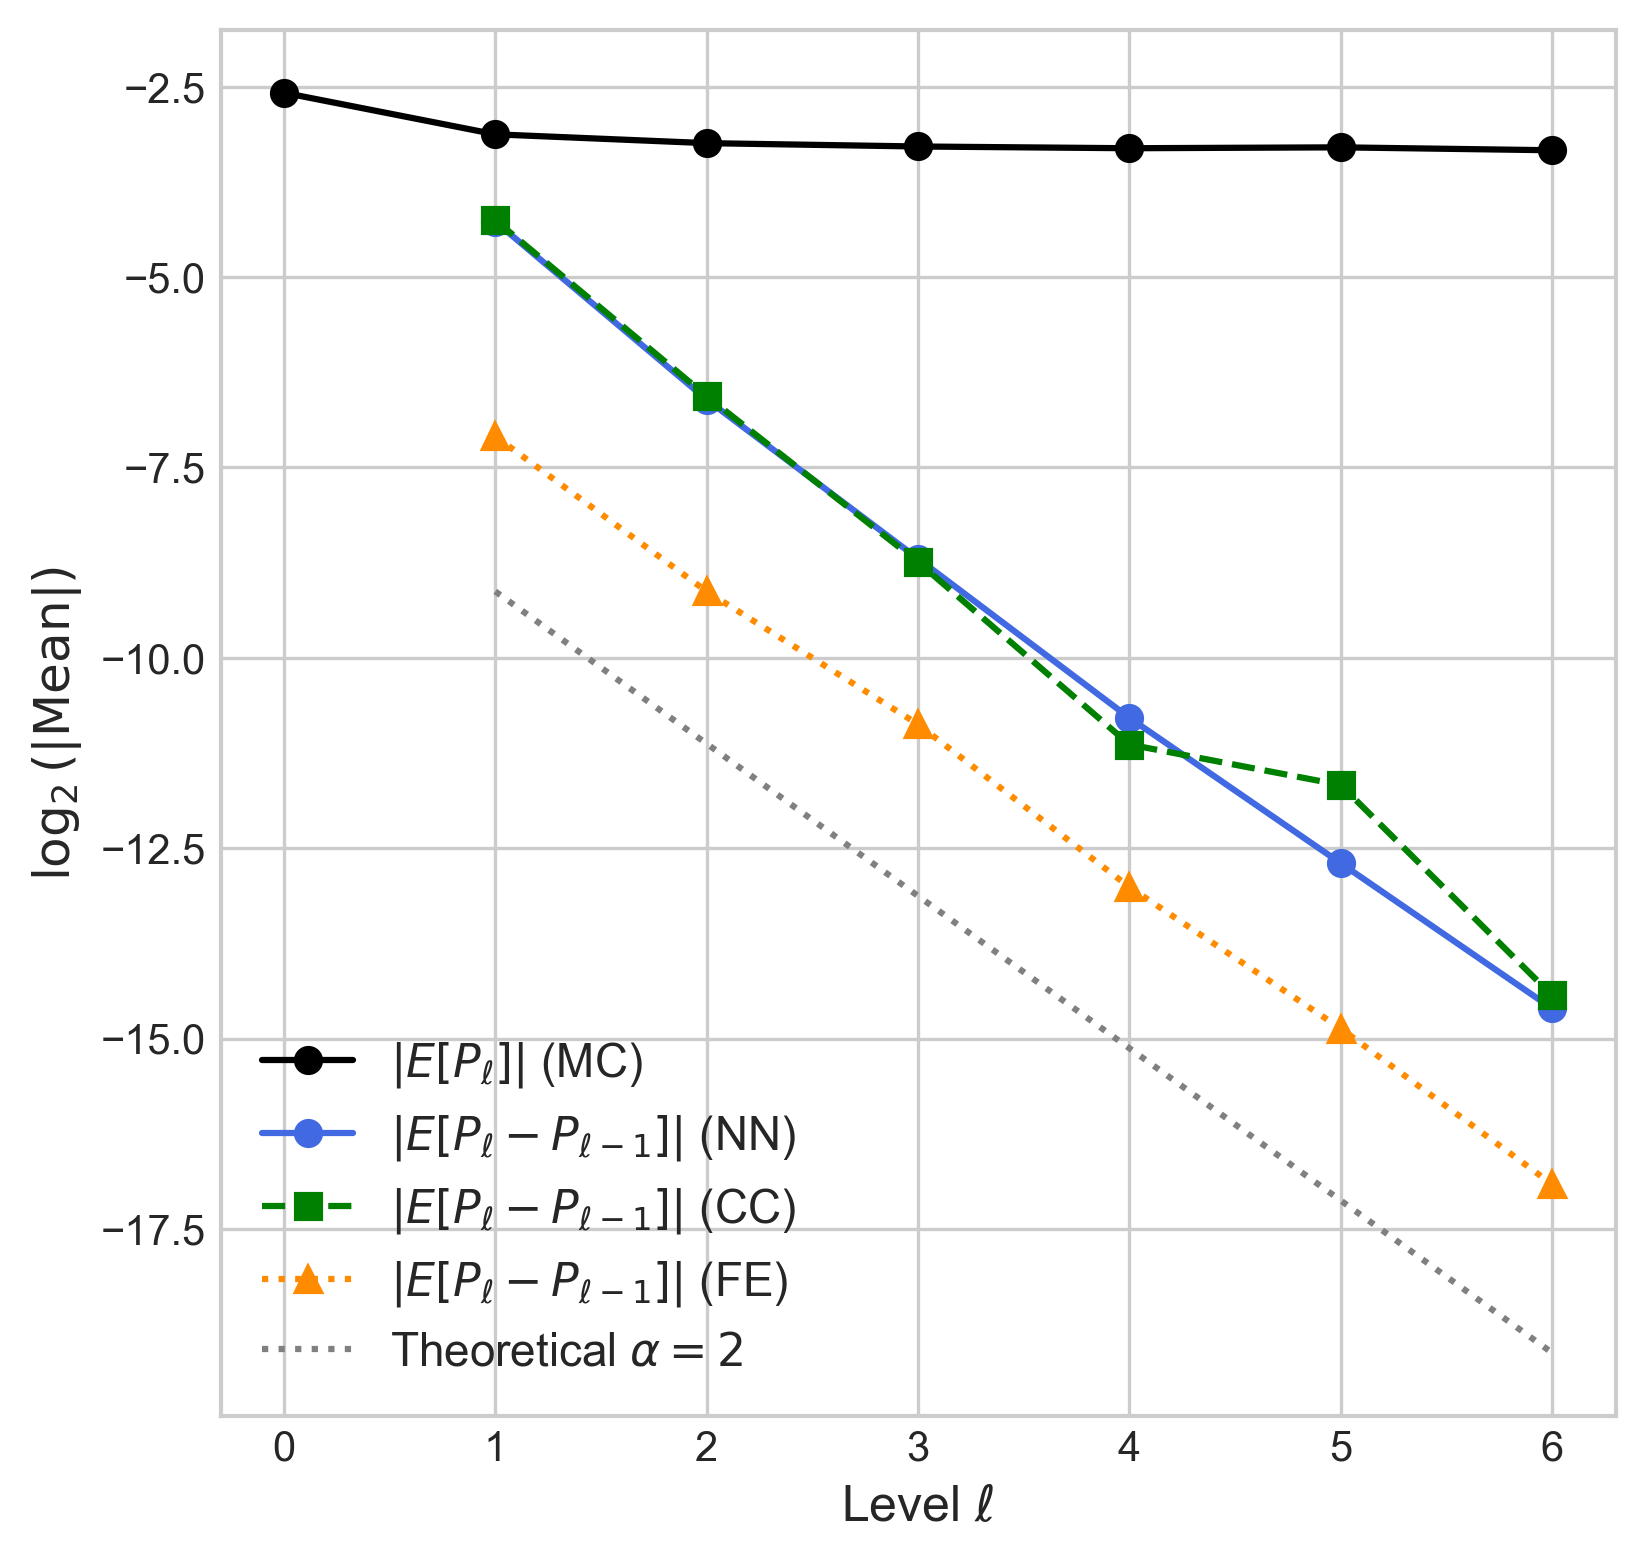
\includegraphics[width=\linewidth]{graphics/she_sq_amp_err_decay.png}
            \caption{Weak error convergence ($\alpha$).}
            \label{fig:she_sq_amp_mean_decay}
        \end{subfigure}
        \hfill
        \begin{subfigure}[b]{0.48\textwidth}
            \centering
            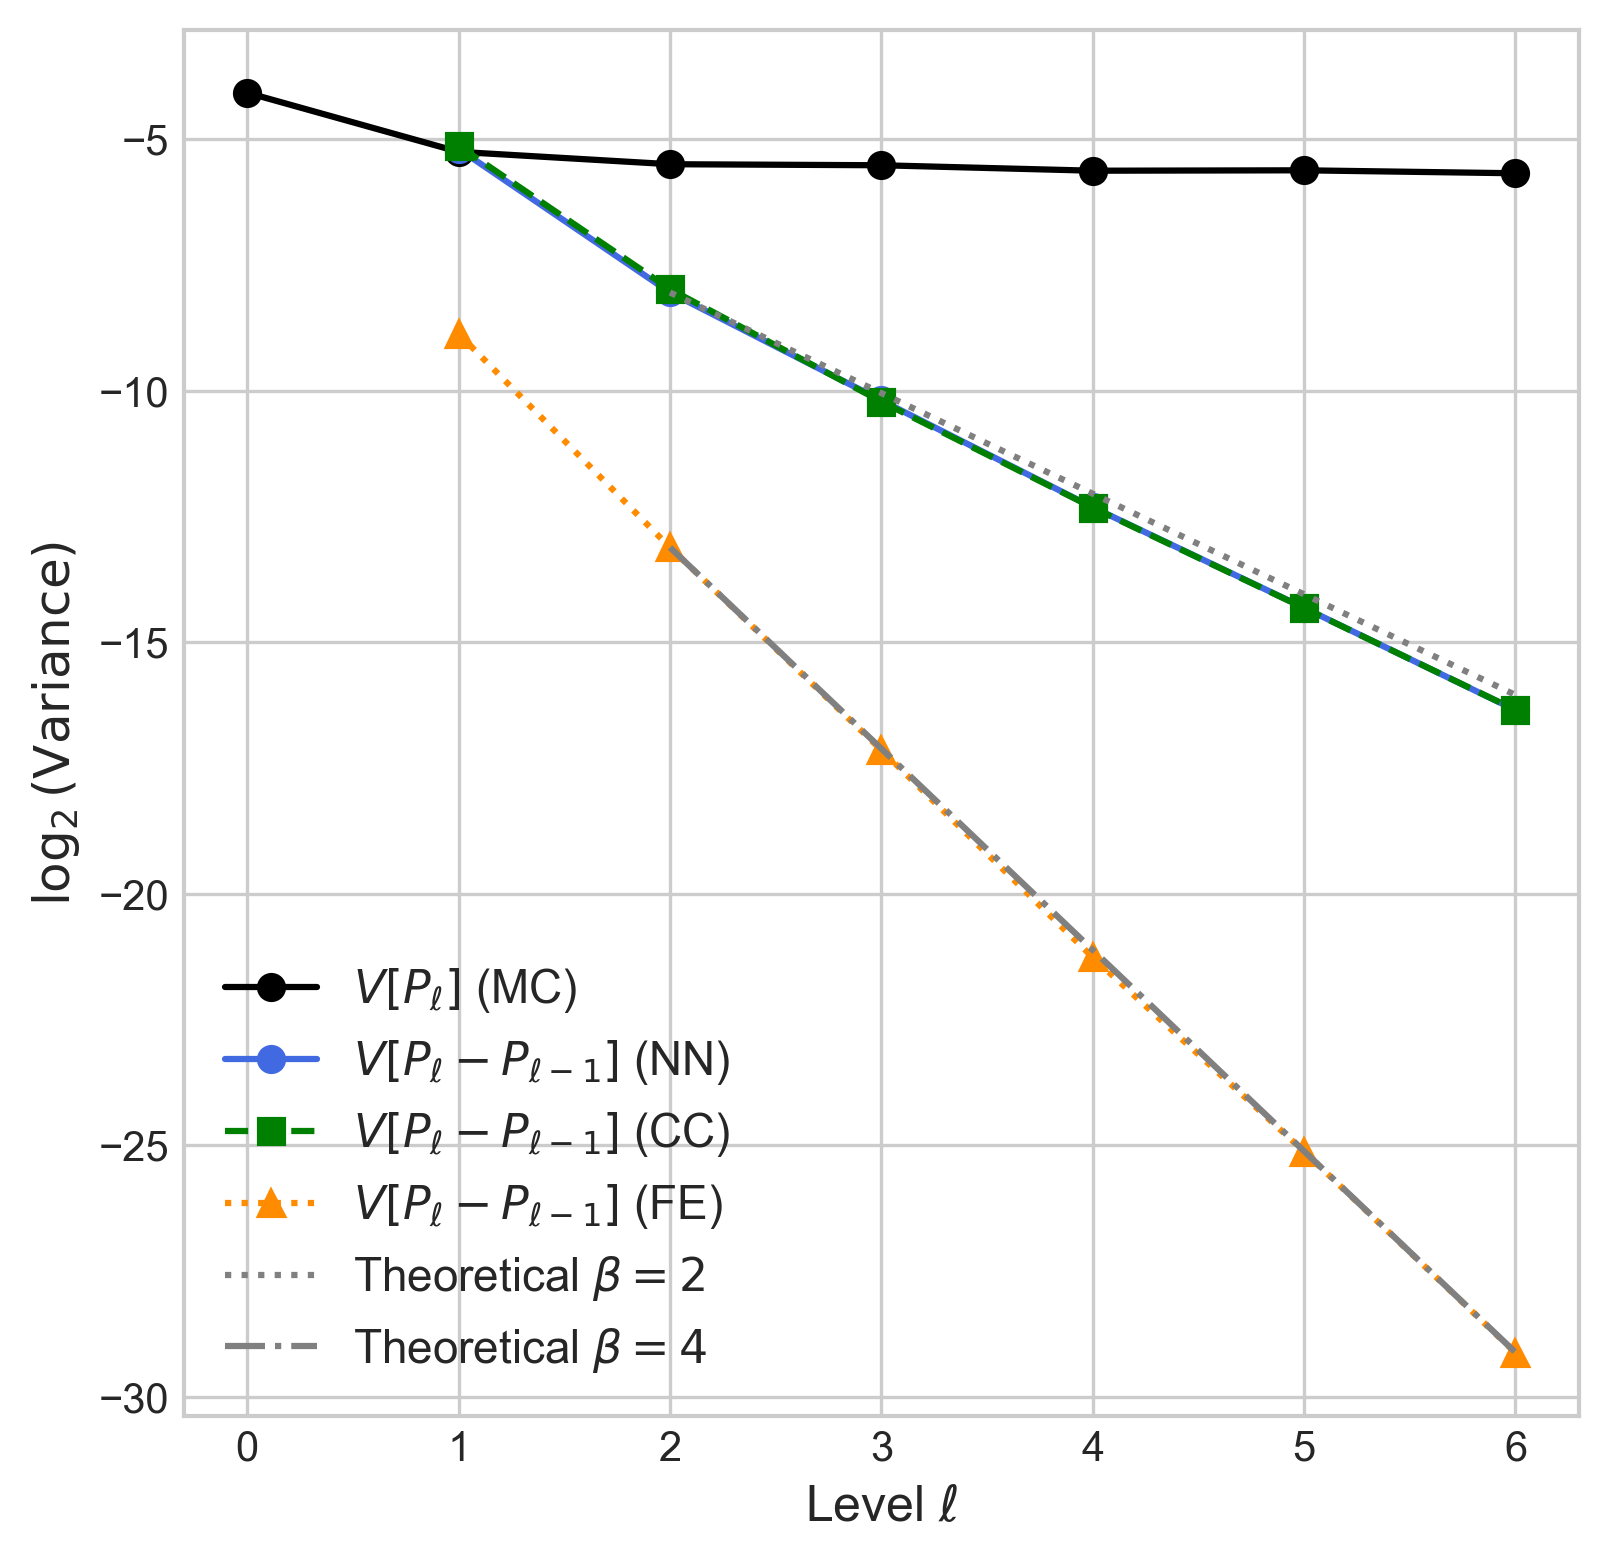
\includegraphics[width=\linewidth]{graphics/she_sq_amp_var_decay.png}
            \caption{MLMC variance decay ($\beta$).}
            \label{fig:she_sq_amp_variance_decay}
        \end{subfigure}        
    \end{subfigure}
    \vspace{1cm}
    \begin{subfigure}{\textwidth}
        \centering
        \begin{subfigure}[b]{\textwidth}
            \centering
            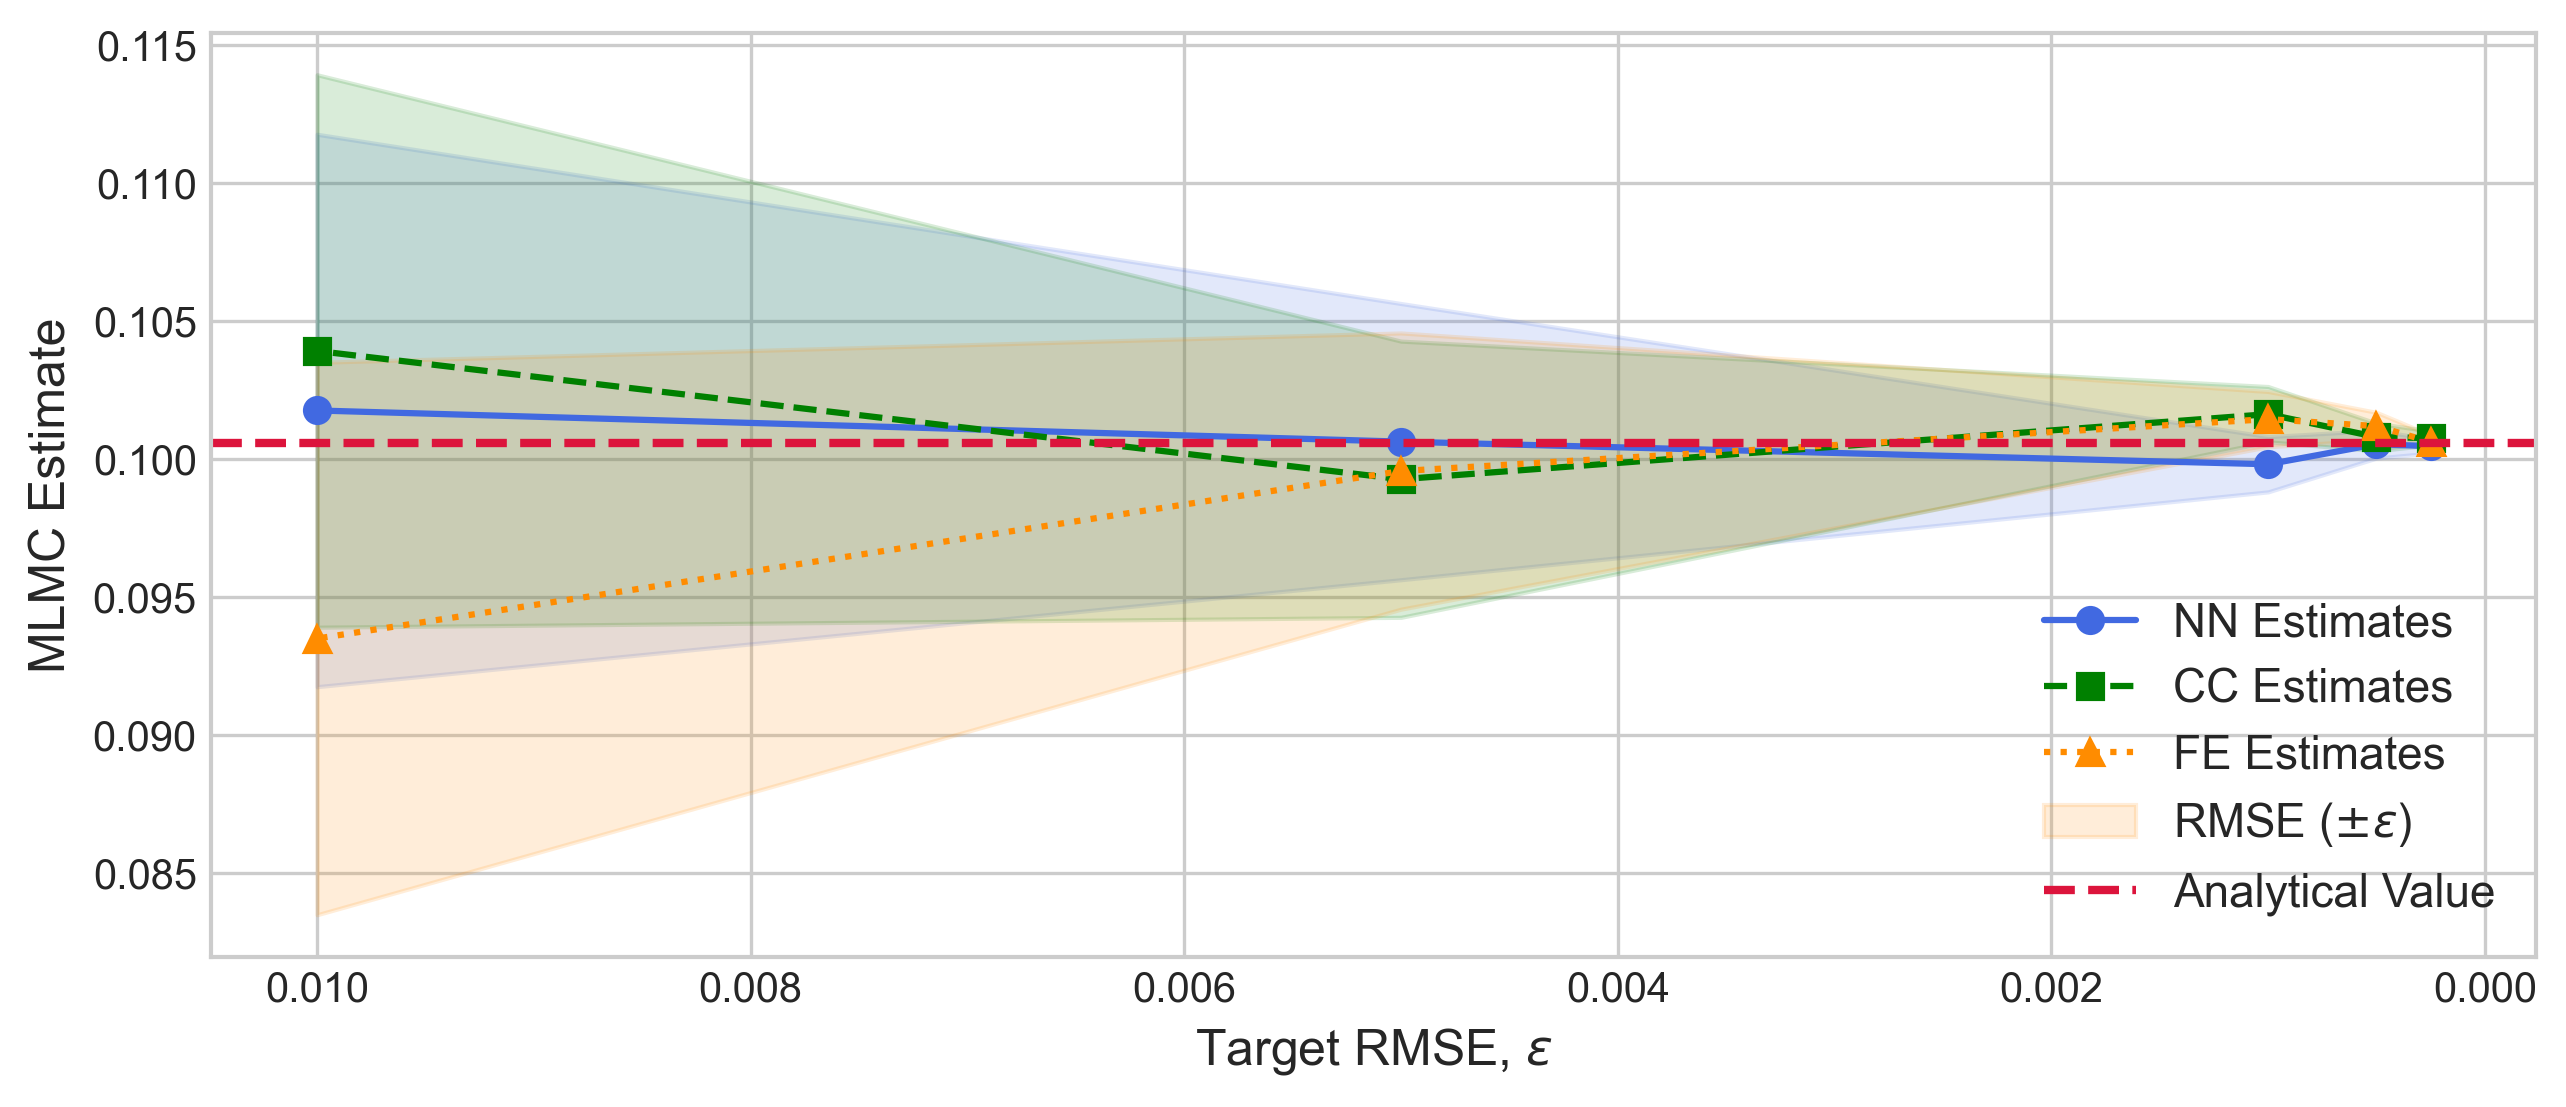
\includegraphics[width=0.7\linewidth]{graphics/she_sq_amp_conv.png}
            \caption{Final MLMC estimate vs. target RMSE ($\varepsilon$).}
            \label{fig:she_sq_amp_conv_vs_eps}
        \end{subfigure}
        \vspace{0.5cm}
        \begin{subfigure}[b]{\textwidth}
            \centering
            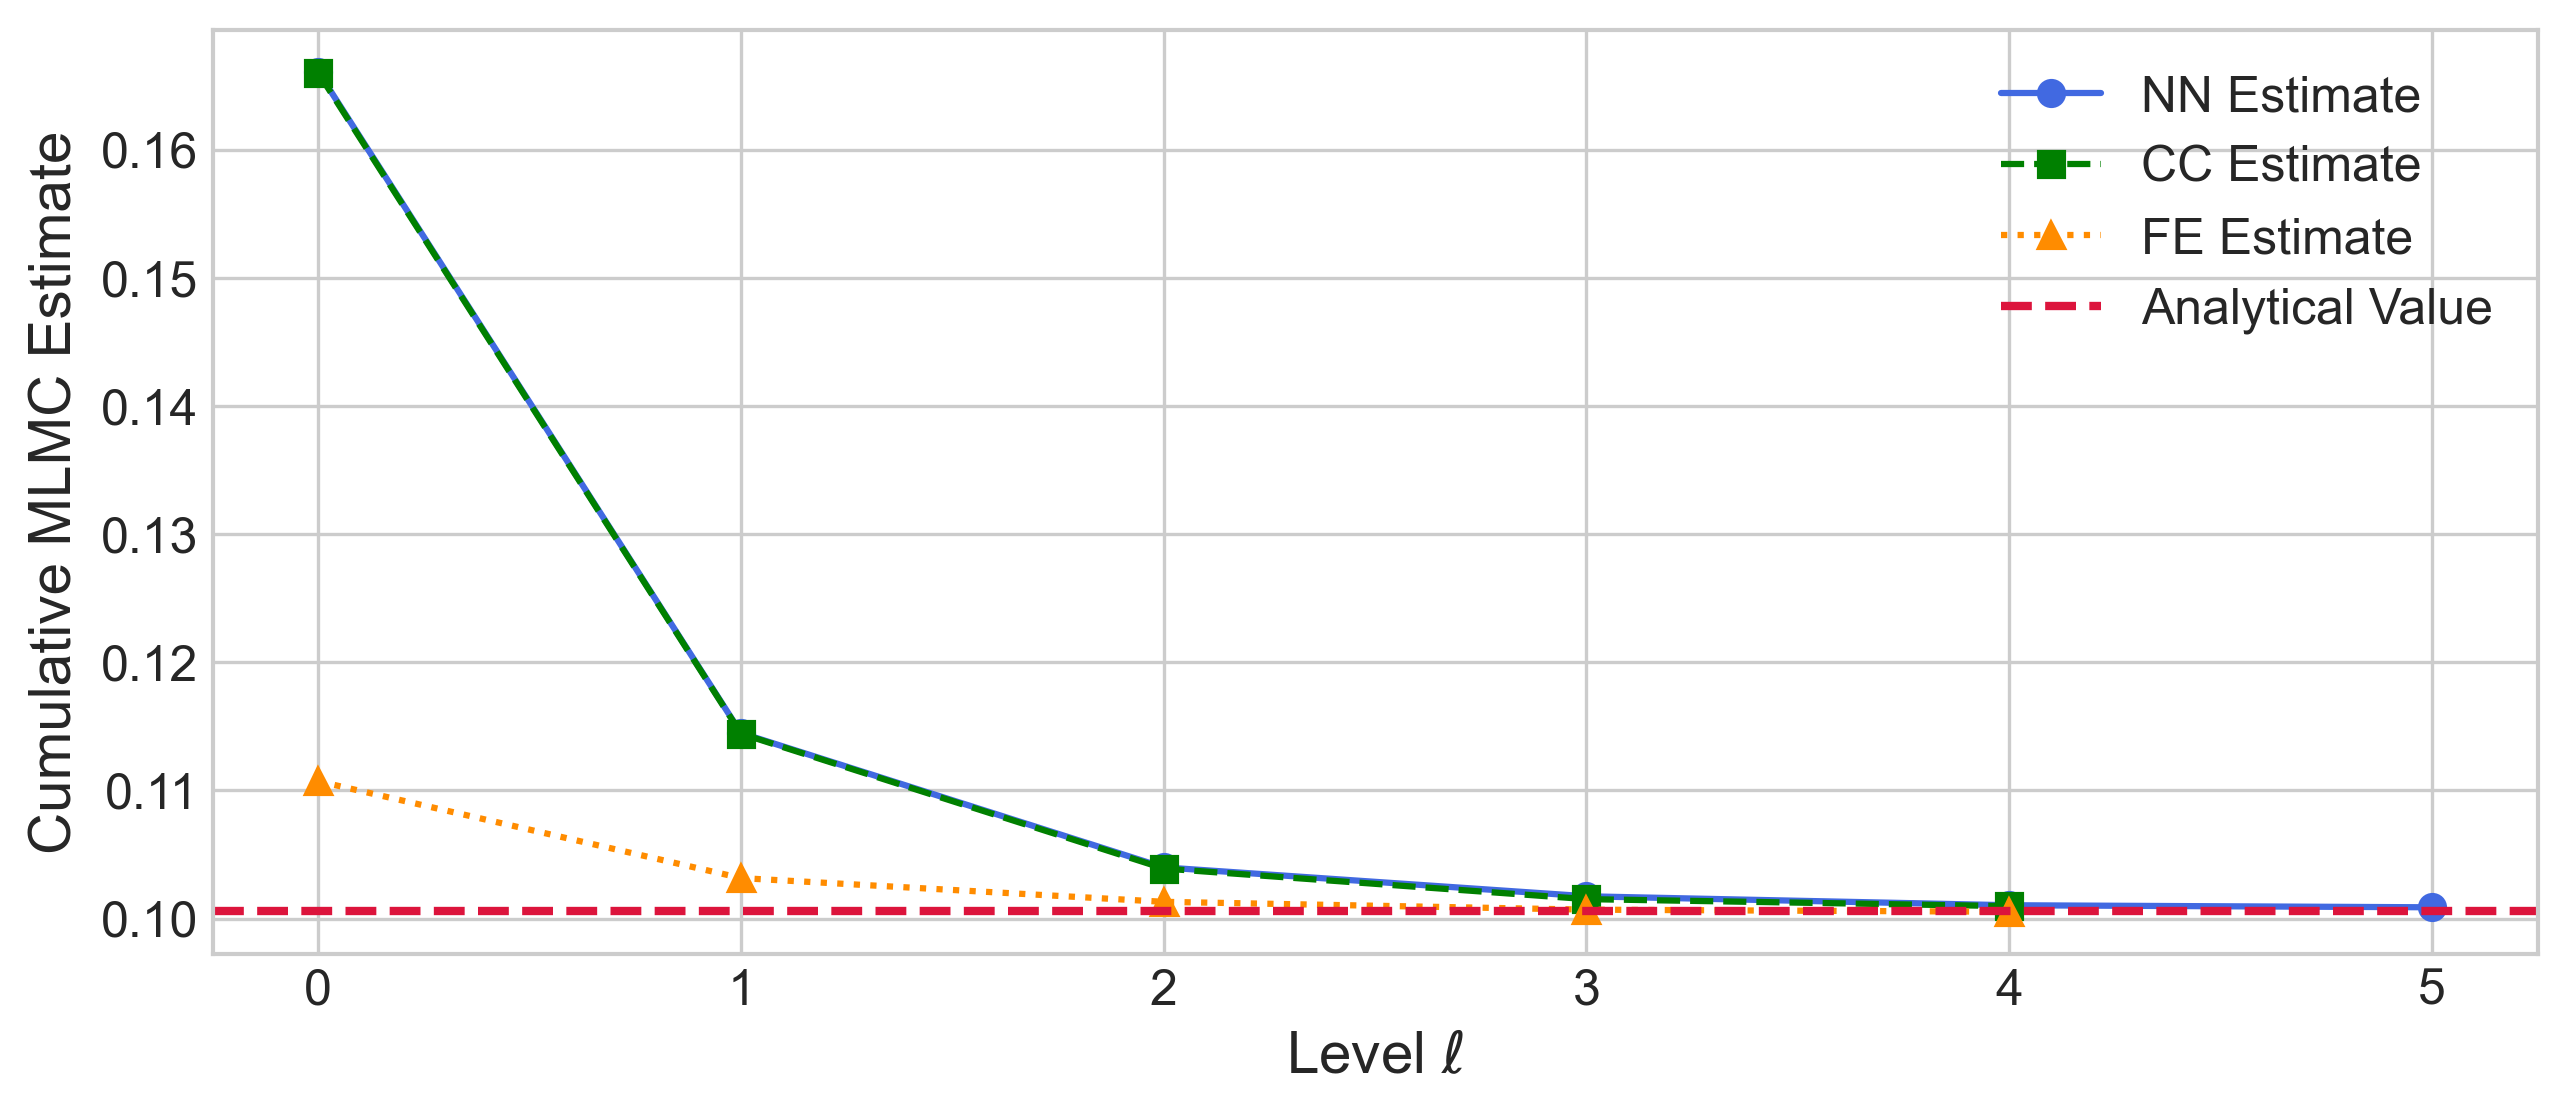
\includegraphics[width=0.7\linewidth]{graphics/she_sq_amp_cumconv.png}
            \caption{Cumulative estimate vs. level ($\ell$) for $\varepsilon=0.001$.}
            \label{fig:she_sq_amp_cumulative_conv}
        \end{subfigure}
    \end{subfigure}
    \caption{Decay and convergence plots for the MLMC implementation of the SHE, using the squared 
    amplitude of the first Fourier mode as our QoI.}
    \label{fig:she_validation_combined}
\end{figure}


We first comment on the rates observed. In line with expectations for a 1D problem, 
we observe $\gamma = 3$ across 
all couplings. Similarly, we obtain estimates of $\alpha = 2$ for all coupling methods,
in line with Proposition \ref{prop:weak_error_for_fourier_mode} which was independent 
of coupling. Figure \ref{fig:she_sq_amp_mean_decay} shows this decay, 
including the theoretical $\alpha=2$ observed rate which can be seen to be in alignment 
with the decays observed. Notably, there is strong alignment in the magnitude of the 
of weak errors for the NN and CC coupling methods, while the FE method systematically has a 
smaller weak error, suggesting fewer samples are required to remove the discretisation 
error for the FE method.

The most critical distinction between the methods is revealed in the variance decay,
shown in Figure \ref{fig:she_sq_amp_variance_decay}. We observe that the FE method
achieves the optimal decay rate of $\beta = 4$, 
We can infer, following 
Proposition \ref{prop:variance_decay_fourier}, that FE coupling achieves 
perfect correlation between levels while the CC method does not. We knew the 
NN method would not, as it discards some noise.

We also include the MC estimator's means and variances, obtained also using $10,000$ samples
at each level reported. We observe no error or variance decay in the MC estimator which 
also aligns with out expectations.

Finally, we observe convergence for all coupling methods. 
Figure \ref{fig:she_sq_amp_conv_vs_eps} shows clear convergence across the different RMSEs chosen. 
In Figure \ref{fig:she_sq_amp_cumulative_conv} we clearly see the benefit of the faster variance decay,
FE coupling requiring only 3 levels to achieve the requisite level of accuracy, while NN and CC 
required 5.


We now provide similar validation results for our SHE MLMC implementation where our QoI is the system energy. 
We have the true value for the problem, $\approx \frac{1}{12}$, via
\ref{eq:she_energy_analytic_soln}.

\begin{table}[htbp]
    \centering
    \begin{tabular}{|l|c|c|r|}
        \hline
        \textbf{Coupling Method} & \textbf{$\alpha$} & \textbf{$\beta$} & \textbf{$\gamma$} \\
        \hline
        Nearest Neighbour & 2.0 & 2.07 & 3.02\\
        Central Coupling & 1.86 & 2.08 & 3.02 \\
        Finite Element & 1.96 & 4.0 & 3.0 \\
        \hline
    \end{tabular}
    \caption{Empirically estimated rates for the system energy}
    \label{tab:energy_decay_rates}
\end{table}

\begin{figure}[htbp]
    \centering
    \begin{subfigure}{\textwidth}
        \centering
        \begin{subfigure}[b]{0.48\textwidth}
            \centering
            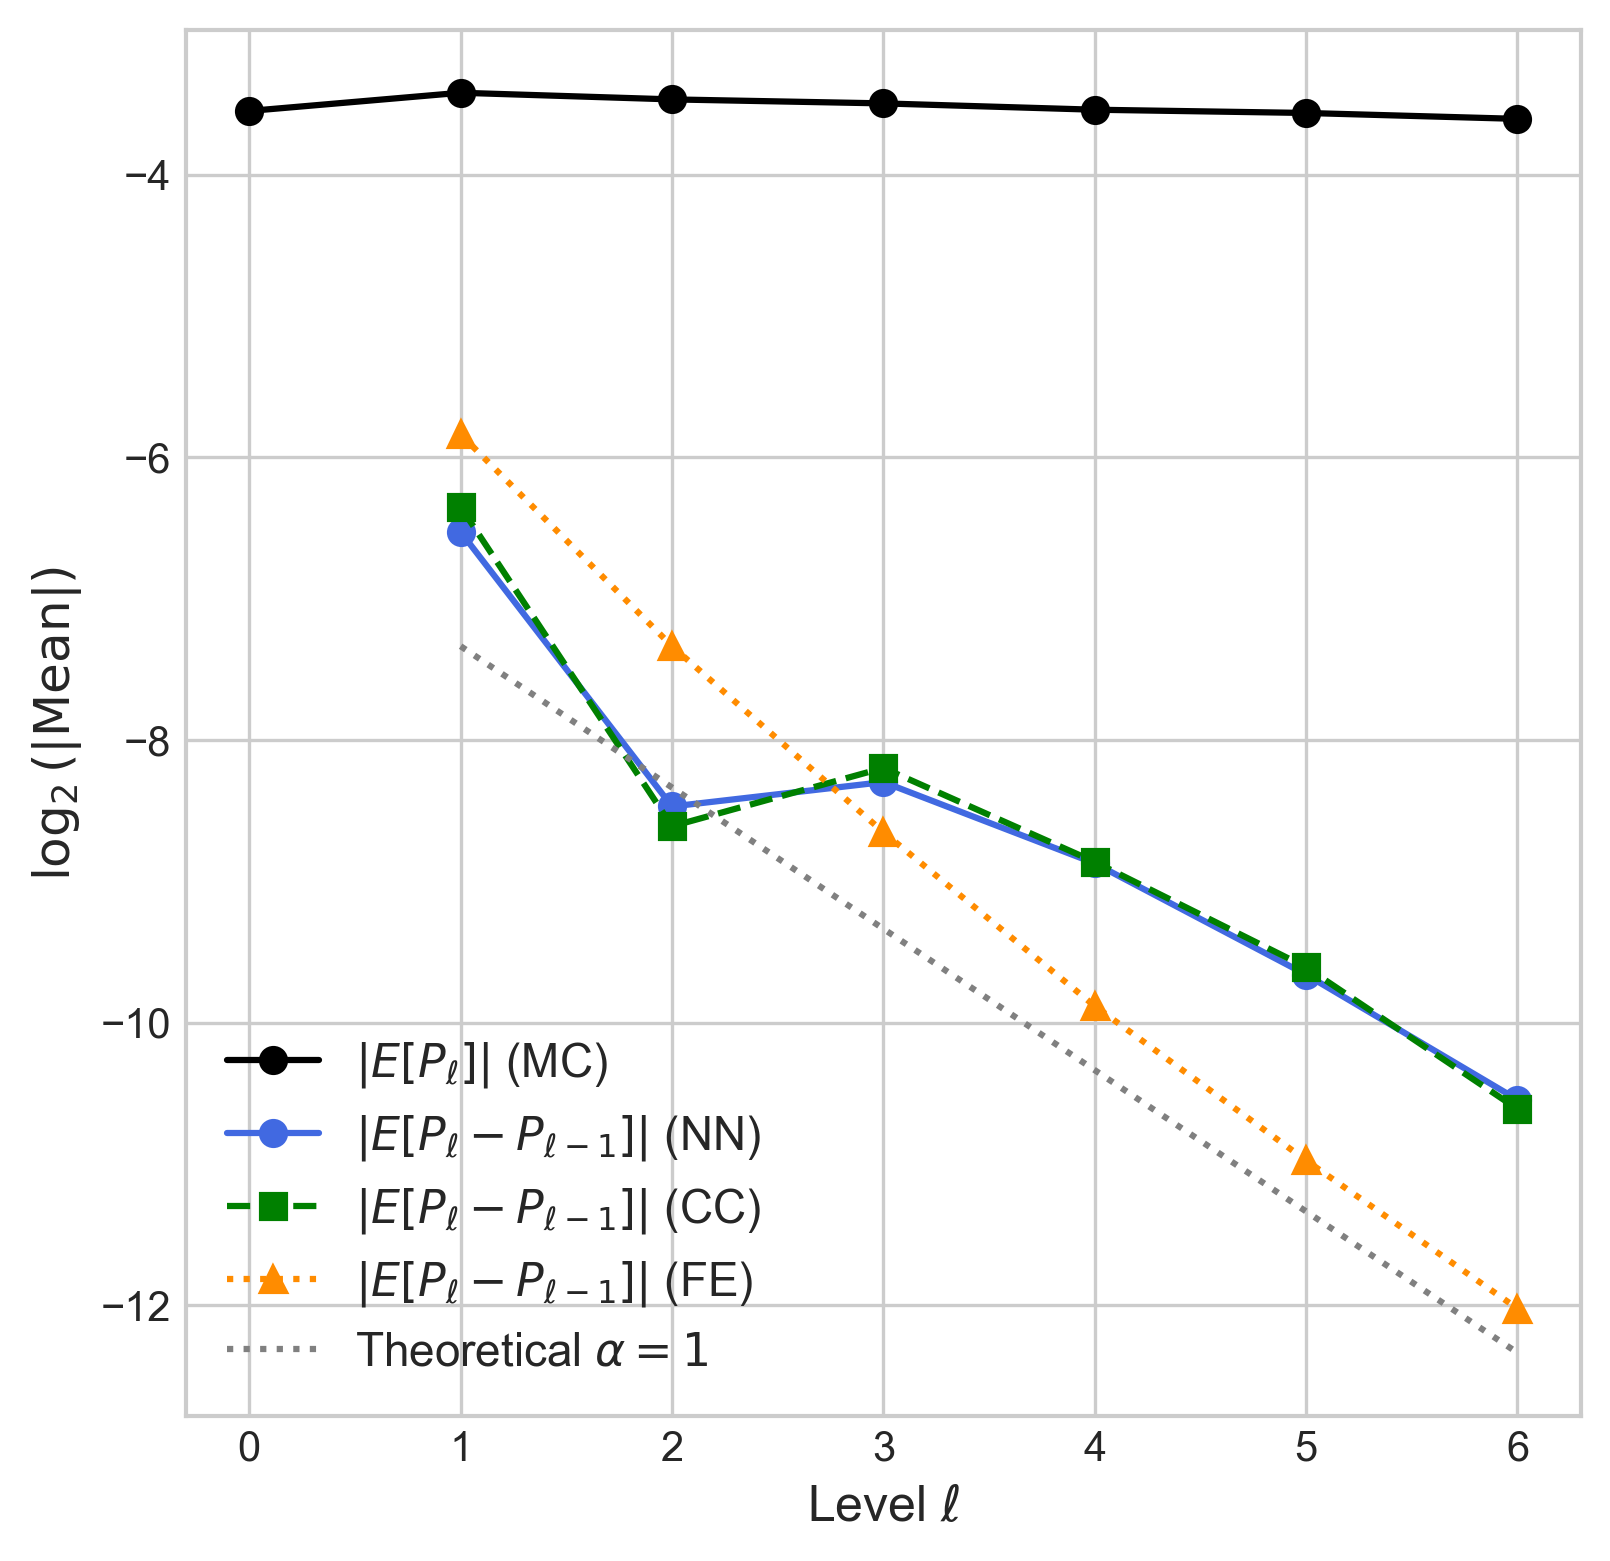
\includegraphics[width=\linewidth]{graphics/she_energy_err_decay.png}
            \caption{Weak error convergence ($\alpha$).}
            \label{fig:energy_mean_decay}
        \end{subfigure}
        \hfill
        \begin{subfigure}[b]{0.48\textwidth}
            \centering
            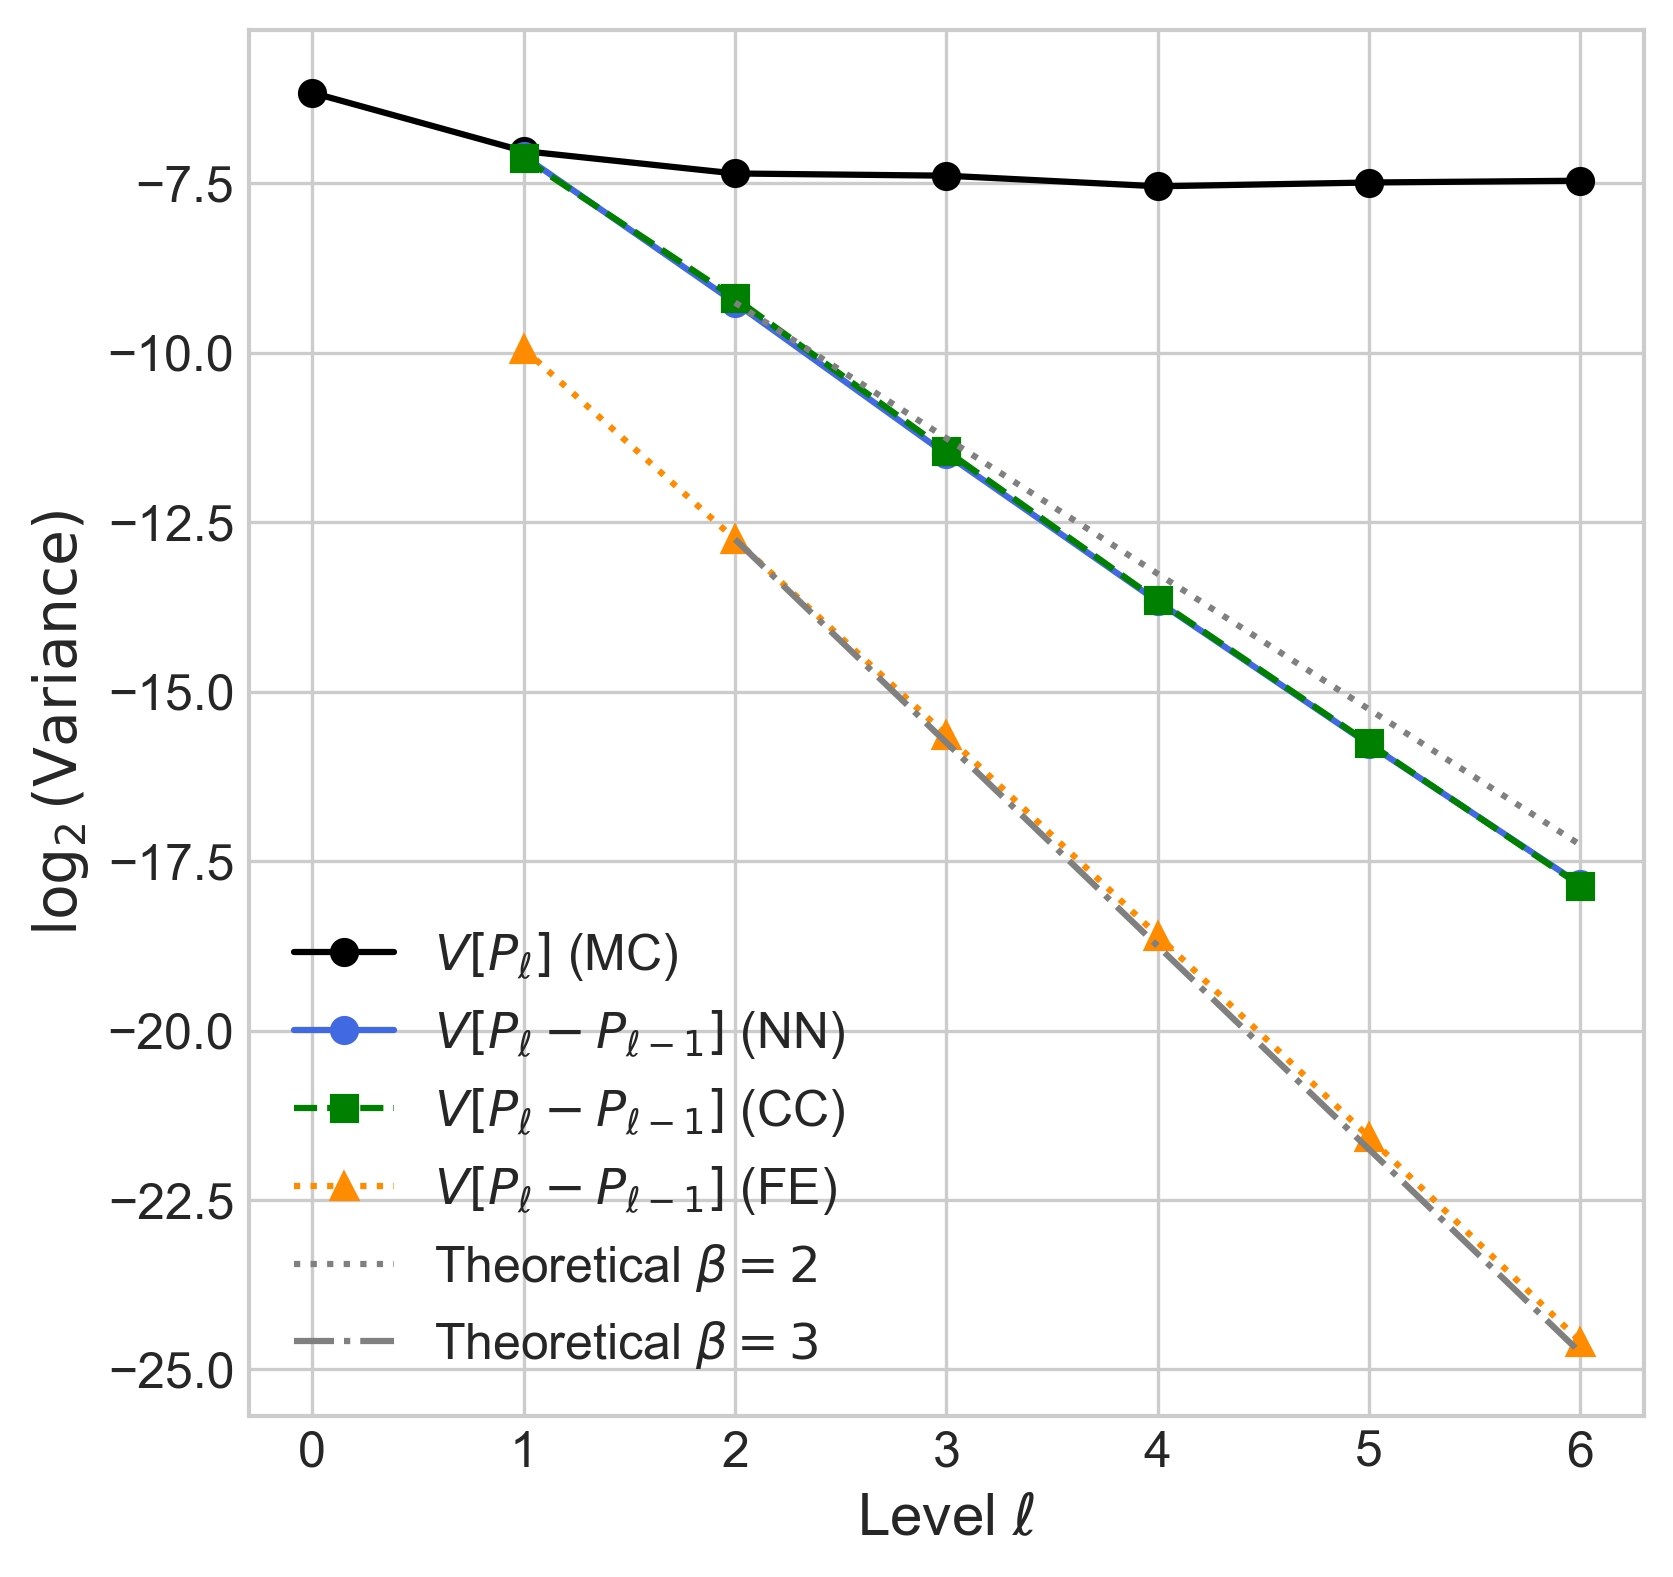
\includegraphics[width=\linewidth]{graphics/she_energy_var_decay.png}
            \caption{MLMC variance decay ($\beta$).}
            \label{fig:energy_variance_decay}
        \end{subfigure}
    \end{subfigure}
    \vspace{1cm}
    \begin{subfigure}{\textwidth}
        \centering
        \begin{subfigure}[b]{\textwidth}
            \centering
            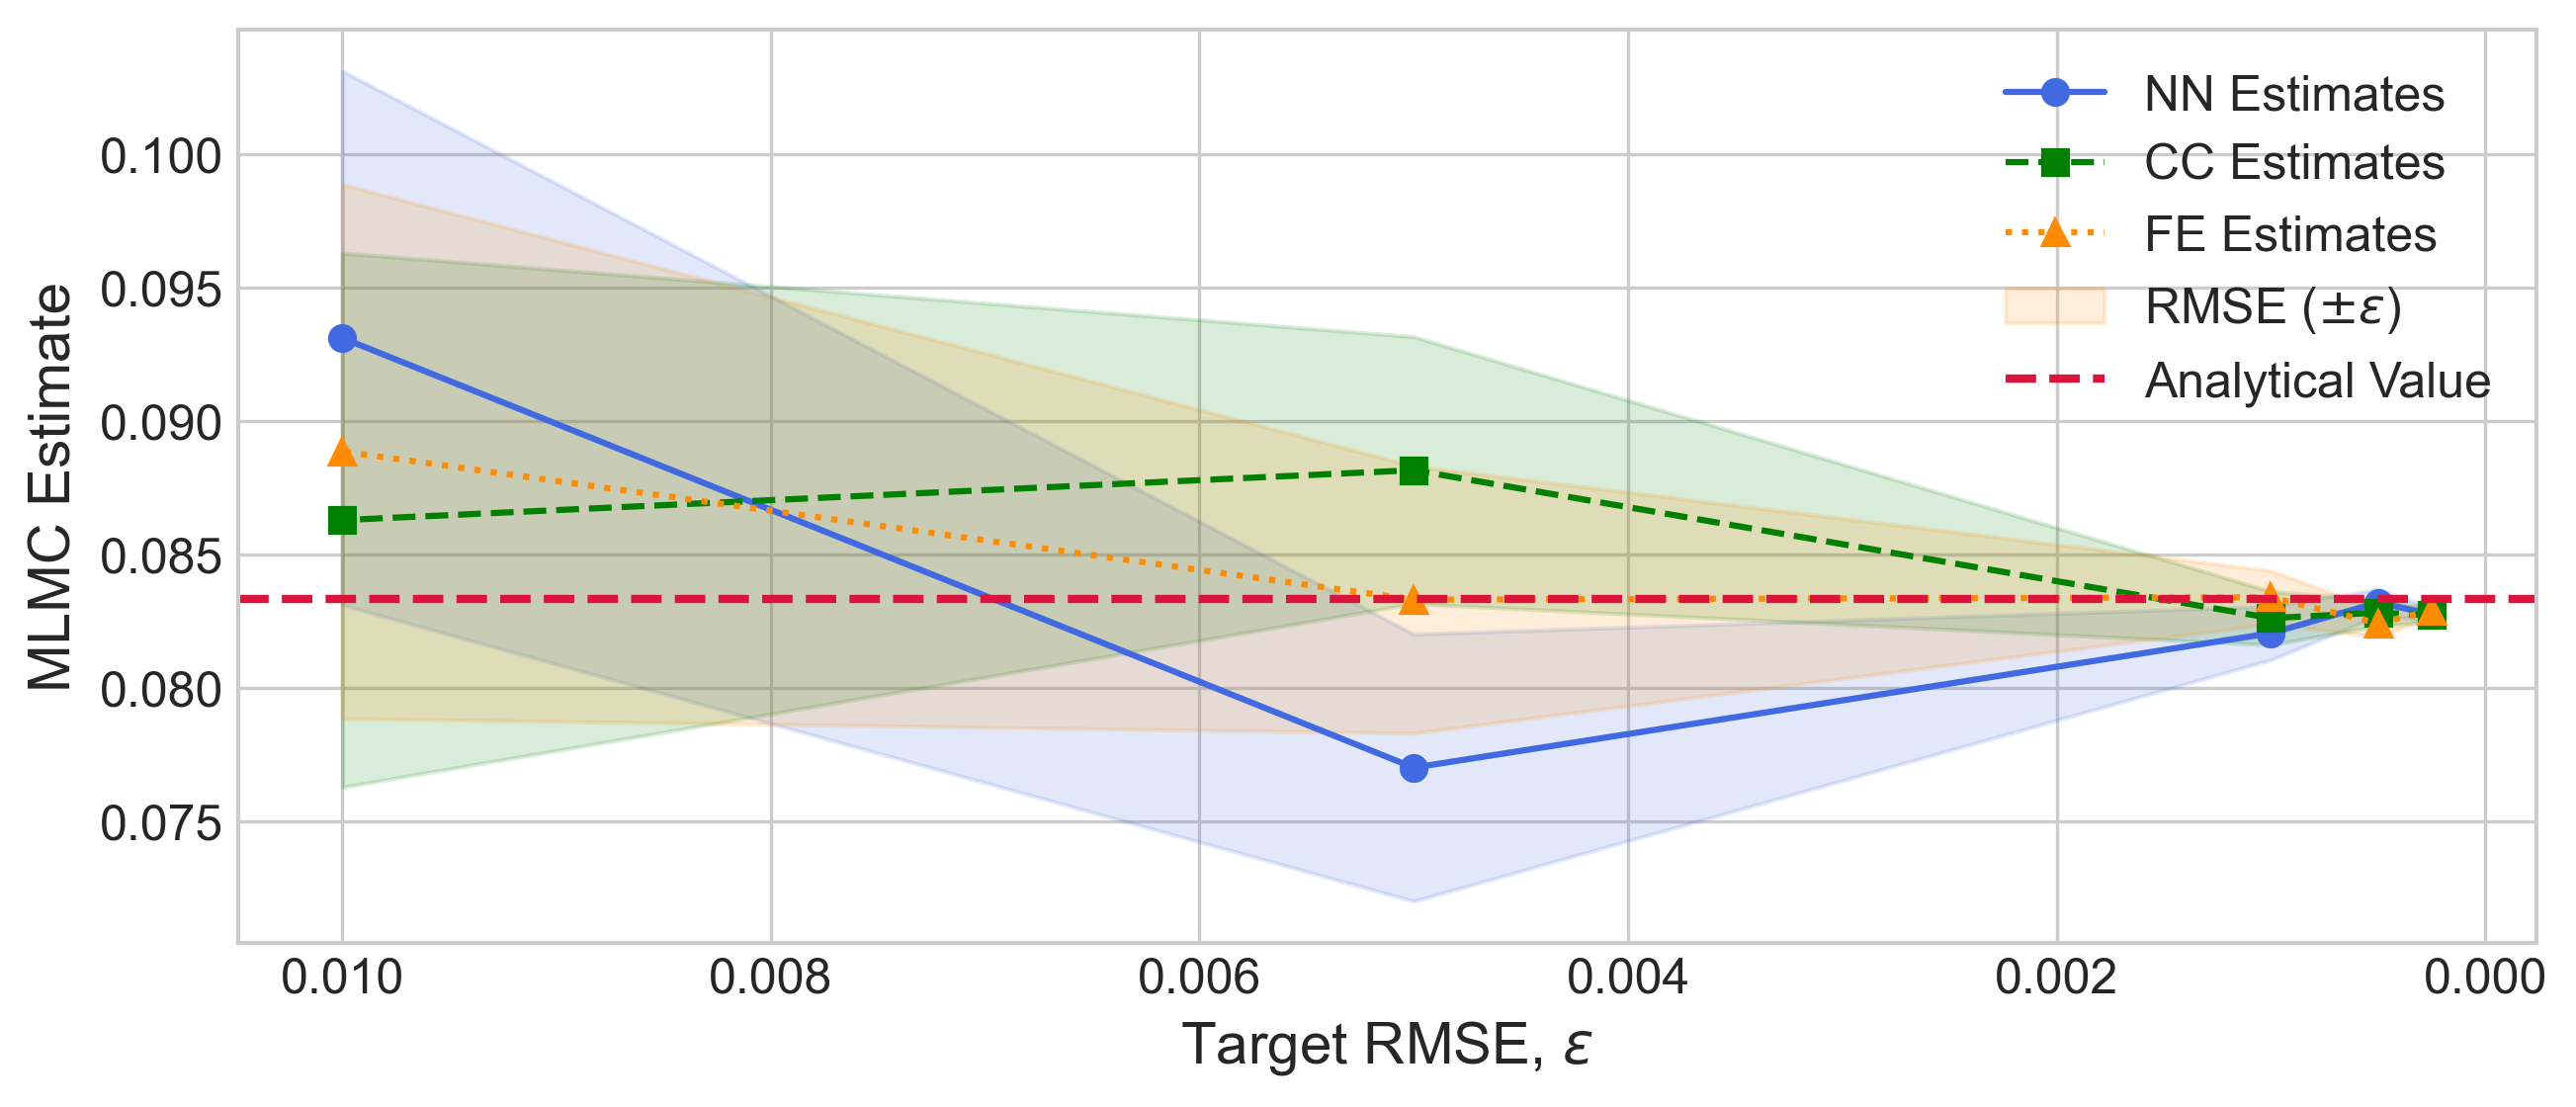
\includegraphics[width=0.7\linewidth]{graphics/she_energy_conv.png}
            \caption{Final MLMC estimate vs. target RMSE ($\varepsilon$).}
            \label{fig:energy_conv_vs_eps}
        \end{subfigure}
        \vspace{0.5cm}
        \begin{subfigure}[b]{\textwidth}
            \centering
            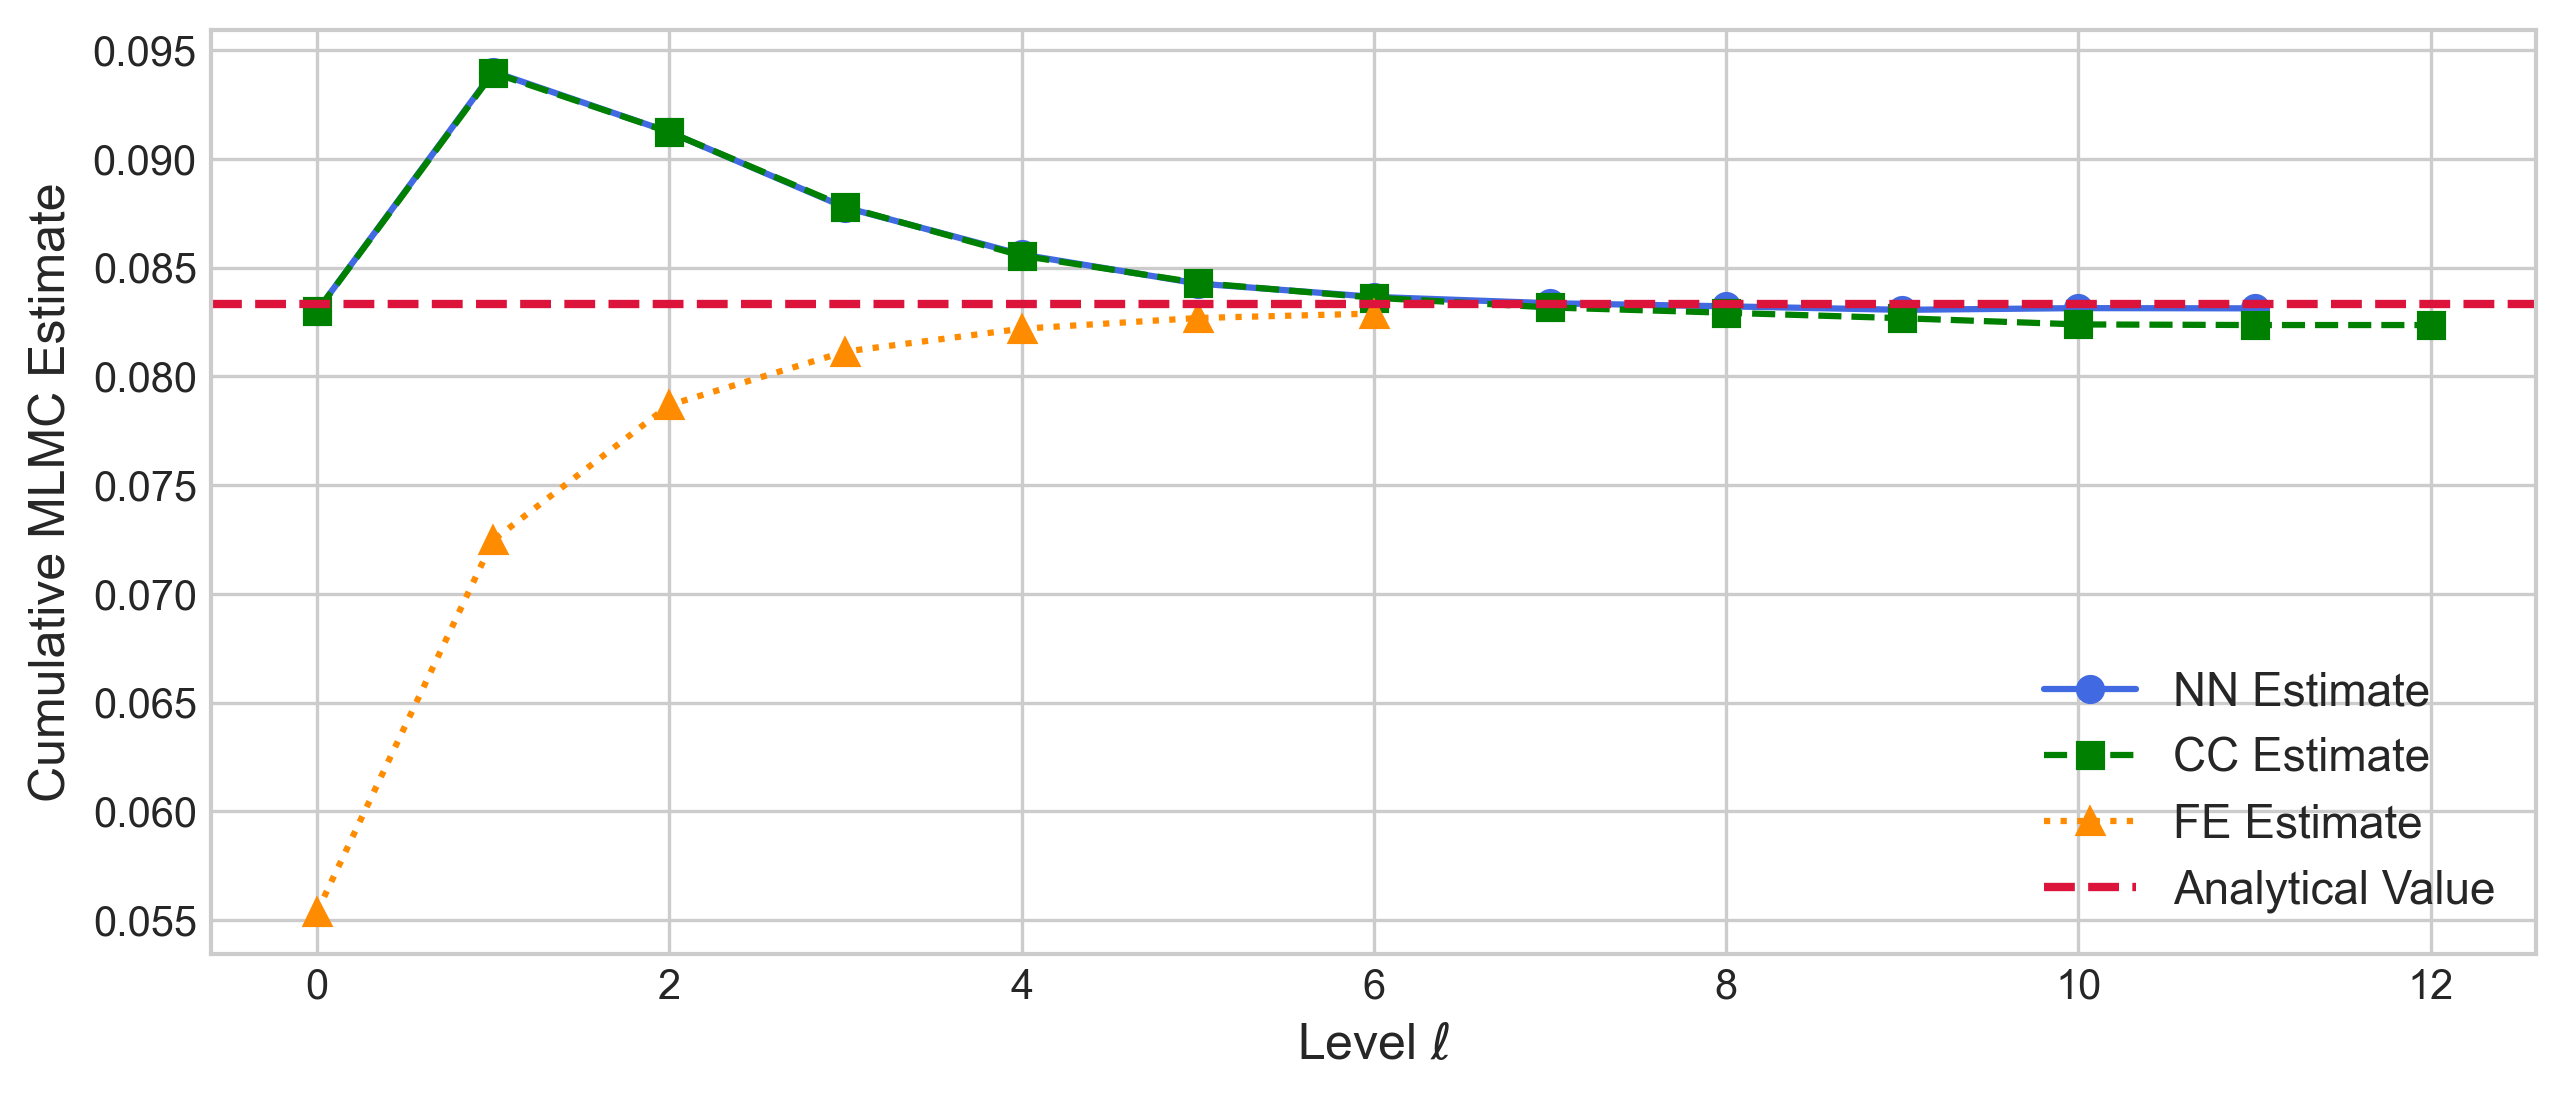
\includegraphics[width=0.7\linewidth]{graphics/she_energy_cumconv.png}
            \caption{Cumulative estimate vs. level ($\ell$) for $\varepsilon=0.001$.}
            \label{fig:energy_cumulative_conv}
        \end{subfigure}
    \end{subfigure}
    \caption{Decay and convergence plots for the MLMC implementation of the SHE, using the system energy as our QoI.}
    \label{fig:she_validation_combined}
\end{figure}

The rates shown in Table \ref{tab:energy_decay_rates} and Figures 
\ref{fig:energy_mean_decay} and \ref{fig:energy_variance_decay} align with the results for the 
squared amplitude. We see the same approximate estimates in the decays. 

In Figure \ref{fig:energy_cumulative_conv} we again see the benefits of the faster 
variance decay, with convergence being achieved at level 6 for the FE method, 
and level 12 for the CC and NN methods.


